\begin{fullwidth}
Welcome to \textit{Development Research in Practice: The DIME Analytics Data Handbook}.
This book is intended to teach all users of development data
how to handle data effectively, efficiently, and ethically.
An empirical revolution has changed the face of development research rapidly over the last decade.
Increasingly, researchers are working not just with complex data,
but with \textit{original} data:
datasets either collected by the research team themselves
or acquired through a unique agreement with a project partner.
Original data, especially if collected or assembled by the team themselves,
requires that the team carefully document how the data was created, handled, and analyzed.
These tasks now contribute as much weight to the quality of the evidence
as the research design and the statistical approaches do.
At the same time, the scope and scale of empirical research projects is expanding:
more people are working on the same data over longer timeframes.
For that reason, the central premise of this book is that data work is a ``social process''.
This means that the many different people on a team need to have the same ideas
about what is to be done, and when and where and by whom,
so that they can collaborate effectively on a large, long-term research project.

\end{fullwidth}

%------------------------------------------------

\section{Who is the team behind this book?}

\textit{Development Research in Practice} shares the lessons, tools,
and processes developed based on DIME's diverse research experience,
and compiles them into a single narrative of best practices for data work.
DIME is the Development Impact Evaluations department of the World Bank.
Its mission is to generate high-quality and operationally relevant data and research
to transform development policy, help reduce extreme poverty, and secure shared prosperity.\cite{legovini2015impact}
DIME develops customized data and evidence ecosystems to produce actionable information
and recommend specific policy pathways to maximize impact.
The department conduct research in 60 countries with 200 agencies, leveraging a
US\$180 million research budget to shape the design and implementation of
US\$18 billion in development finance.
DIME also provides advisory services to 30 multilateral and bilateral development agencies.
The DIME team includes four primary topic pillars:
Economic Transformation and Growth;
Gender, Economic Opportunity, and Fragility;
Governance and Institution Building;
and Infrastructure and Climate Change.
Over the years, DIME has employed dozens of research economists,
and hundreds of full-time research assistants, field coordinators, and other staff.
The team has conducted over 325 impact evaluations.
This book exists to take advantage of that concentration and scale of research,
to synthesize many resources for data collection and research,
and to make DIME tools available to the larger community of development researchers.

As part of its broader mission, DIME invests in public goods
to improve the quality and reproducibility of development research around the world.
One key early innovation at DIME was the creation of DIME Analytics,
the team responsible for writing and maintaining this book.
DIME Analytics is a centralized unit that develops and ensures adoption
of high quality research practices across the department's portfolio.
This is done through an intensive, collaborative innovation cycle:
DIME Analytics onboards and supports research assistants and field coordinators,
provides standard tools and workflows to all teams,
delivers hands-on support when new tasks or challenges arise,
and then develops and integrates lessons from those engagements to bring to the full team.
Resources developed and tested in DIME are converted into public goods
for the global research community, through open-access trainings and open-source tools.

\textit{Development Research in Practice} is not sector-specific;
it will not teach you econometrics,
or how to design an impact evaluation.
There are many excellent existing resources on those topics.
Instead, this book will teach you how to think about all aspects of your research from a data perspective,
how to structure research projects to maximize data quality,
and how to institute transparent and reproducible workflows.



%------------------------------------------------

\section{How to read this book}

This book aims to be a highly practical resource so the reader can
immediately begin to collaborate more effectively
on large, long-term research projects
that use the methods and tools discussed in it.
This introduction will outline the basic philosophies
that motivate this book and our approach to research data.
Before you begin reading the main chapters,
you should be aware of our mindset
that research data work is primarily about
communicating within a team
and that standardization and simplification of data tasks
is a major enabler of effective collaboration.
The rest of the book will walk you through data work at each stage
of an empirical research project, from design to publication.
Each chapter focuses on a single stage in the data work process.

\textbf{Chapter 1} outlines a set of practices and ideals that help to ensure that
research consumers can be confident in the conclusions reached,
and research work can be assumed and verified to be reliable.
It begins with ethical principles to guide empirical research,
focusing on research reproducibility, transparency, and credibility.
It also introduces tools that are used to document
the aims and methods of a research project,
ensuring that meta-information about your research is available
and that you approach all data work with an eye towards the future.

\textbf{Chapter 2} will teach you to structure your data work for collaborative research,
while ensuring the privacy and security of research participants.
It discusses the importance of planning the tools that will be used;
lays the groundwork to structure the research project at its outset --
long before any data is acquired --
and provides suggestions for collaborative workflows and tools.
It also describes essential ethical practices around data,
as well as common pitfalls in legal and practical management of data
that respect the rights of research participants.

\textbf{Chapter 3} turns to the measurement framework,
a special set of information that describes the data in your project
and how you plan to use it.
Setting up a measurement framework means translating a research design to a data work plan,
including master datasets that are appropriate to the design,
tracking and monitoring field work across time,
and implementing and evaluating experimental designs in a rigorous manner.

\textbf{Chapter 4} covers data acquisition. We start with
the legal and institutional frameworks for data ownership and licensing,
to ensure that you are aware of the rights and responsibilities
of using data collected by you or by others.
We provide a deep dive on collecting high-quality primary electronic survey data,
including developing and deployting survey instruments.
Finally, we discuss secure data handling during transfer, sharing, and storage,
which is essential in protecting the privacy of respondents in any data.

\textbf{Chapter 5} describes workflows for data processing.
It details how to construct ``tidy'' data at the appropriate units of analysis,
how to ensure uniquely identified datasets, and
how to routinely incorporate data quality checks into the workflow.
It also provides guidance on de-identification and cleaning of personally-identified data,
focusing on how to understand and structure data
so that it is ready for indicator construction and analytical work.

\textbf{Chapter 6} discusses data analysis.
It begins with data construction, or the creation of new variables
from the raw data acquired or collected in the field.
It introduces core principles for writing analytical code
and creating, exporting, and storing research outputs
such as figures and tables reproducibily using dynamic documents.

\textbf{Chapter 7} turns to publication of research outputs,
including manuscripts, code, and data.
This chapter discusses
how to effectively collaborate on technical writing
using {\LaTeX} as a document preparation system.
It covers how and why to release or publish datasets
in an accessible, citable, and safe fashion.
Finally, it provides guidelines for preparing
functional and informative reproducibility packages
that contain all the code, data, and meta-information needed
for others to evaluate and reproduce your work.

\begin{fullwidth}
\begin{figure}
	\centering
	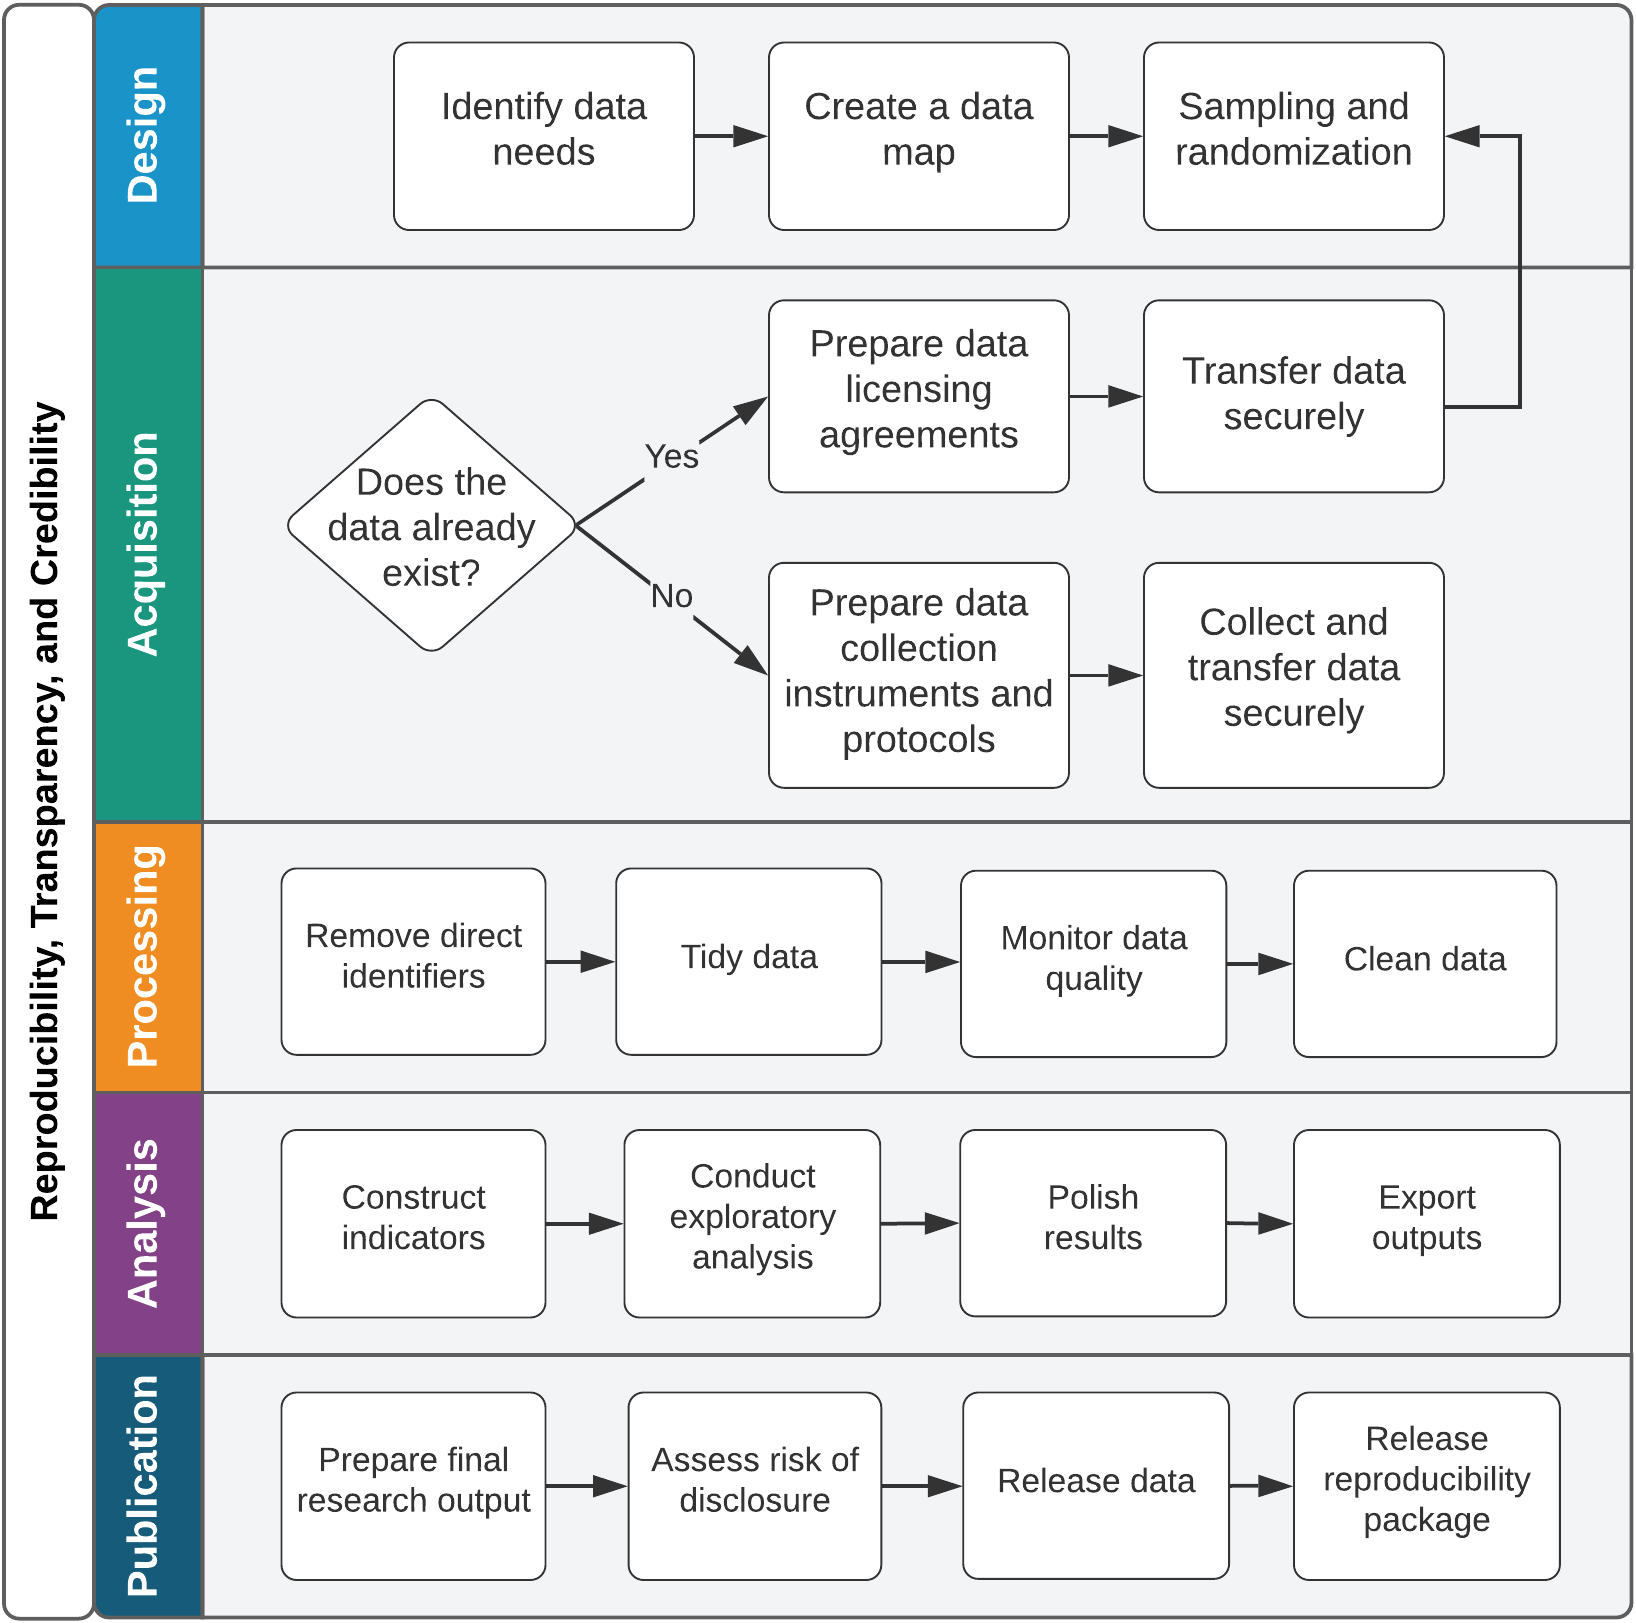
\includegraphics[width=1.25\linewidth]{diagrams/Intro}
	\caption{}
	\label{fig:intro}
\end{figure}
\end{fullwidth}

After reading each chapter, you should understand
what tasks your team will be performing,
where in the data workflow each task falls,
and how to implement them according to best practices.
You should also understand how the various stages tie together,
and what inputs and outputs are required from each.
Then, the references and links contained in each chapter
will lead you to detailed descriptions of individual
ideas, tools, and processes when you need to implement the tasks yourself.
In particular, highly specific implementation details
will often be found on the \textbf{DIME Wiki}.\sidenote{Like this:
	\url{https://dimewiki.worldbank.org/Primary_Data_Collection}}

The DIME Wiki is one of DIME Analytics' flagship products,
a free online collection of our resources and best practices.\sidenote{
	\url{https://dimewiki.worldbank.org}}
This book complements the DIME Wiki by providing a structured narrative
of the data workflow for a typical research project.
The Wiki, by contrast, provides unstructured but detailed and up-to-date information
on how to complete each task, and links to further practical resources.
For some implementation portions where precise code is particularly important,
we provide minimal code examples either in the book or on the DIME Wiki.
All code guidance is software-agnostic, but code examples are provided in Stata.

%------------------------------------------------
\section{Handling original data is a core research task}

In the past, data work was often treated as a ``black box'' in research.
A published manuscript might exhaustively detail
research designs, estimation strategies, and theoretical frameworks,
but would typically reserve very little space for detailed descriptions
of how data was actually collected and handled.
Not only is it almost impossible to assess the quality of the data in such a paper,
it is very hard for research teams -- particularly new staff --
to understand and learn the skills and tools needed to do this well.
There are few guides to the conventions, standards, and best practices
that are fast becoming a necessity for empirical research.
Since 2010, reproducibility practices in development have been rapidly adopted,\cite{swanson2020research}
in part due to increasing requirements by publishers and funders to release code and data.
However, little practical guidance on complete data handling workflows are available for practitioners,
aside from one relatively recent handbook on reproducibility.\cite{christensen2019transparent}
This book aims to fill that gap,
covering data workflows at all stages of the research process,
from design to data acquisition and analysis.

The Analytics team has invested many hours over many years
learning from data work across DIME's portfolio,
identifying inefficiencies and barriers to success,
developing tools and trainings, and standardizing best-practice workflows adopted in DIME projects.
It has also invested significant energy in the language and materials
used to teach these workflows to new team members,
and, in many cases, in software tools that support these workflows explicitly.
DIME team members often work on diverse portfolios of projects
with a wide range of teammates, and we have found
that standardizing core processes across all projects
results in higher-quality work with fewer opportunities to make mistakes.
In that way, the Analytics team is DIME's method of ``institutionalizing''
tools and practices, developed and refined over time,
that give the department a common base of knowledge and practice.
In 2018, for example, DIME adoped universal reproducibility checks
conducted by the Analytics team;
the lessons from this practice helped move the DIME team
from where 50\% of submitted papers in 2018
required significant revision to pass
to where 64\% of papers passed in 2019 without revision required.

Data handling and documentation is a key skill for researchers and research staff,
whether data is collected through surveys, shared by partner organizations,
or acquired from ``big'' data sources like sensors, satellites, or call data records.
Standard processes and documentation practices
are important throughout the research process to accurately convey
and implement the intended research design.\cite{vilhuber_lars_2020_3911311}
For example, statistical code is typically an essential part of
research design components such as sampling, randomization, and power analysis.
As data is obtained, its quality must be validated,
linkages between datasets must be organized and managed,
and errors must be identified and corrected.
Once raw data is in hand, researchers must create and analyze the
outcome measures of interest for the research study;
then they must conduct the actual analyses.
When these are done in an ad-hoc or project-specific manner,
it is very difficult for others to understand what is being done --
in that case, a reader has to simply trust that the author did these things right.
Standardizing and documenting these processes
makes it possible to evaluate and understand
the exact details of each step of this work
alongside any final research outputs.

Researchers therefore need to maintain records of the handling and processing of all their data,
which involves managing and collating different types of information,
often at different levels of analysis and different stages in time.
The tight linkages between documentation, data quality, and policy decisions
have long been recognized by research entities such as government statistical agencies,\cite{jepdataquality}
and must now be imported into the practice of researchers who collect original data
rather than relying on data that comes from, for example, highly-experienced statistical agencies.

A breakdown in any part of this data pipeline
means that the results that are acquired become unreliable.\cite{mccullough2008economics}
If that happens, the results cannot be faithfully interpreted
as being an accurate picture of the intended research design.\sidenote{
  \url{https://blogs.worldbank.org/impactevaluations/more-replication-economics}}
Because we almost never have ``laboratory'' settings\sidenote{
  See \citet{baldwin2015elections} for an example.}
in this type of research,
such a failure has a very high cost:
we will have wasted the investments that were made into knowledge generation,
and the research opportunity itself,
where we intended to conduct the study.\cite{camerer2016evaluating}
Hence accurate and reproducible data management and analysis
is essential to the success and credibility of modern research.

\section{Documenting data work with standardized code}

One method of solving this problem in the social context
is what we refer to as \textbf{process standardization}.
Process standardization means that there is
little ambiguity about how something ought to be done,
and therefore the tools to do it can be set in advance.
Standard processes help other people understand your work.
Work should be well-documented in the sense that others can:
(1) quickly understand what a particular process or output is supposed to be doing;
(2) evaluate whether or not it does that thing correctly; and
(3) modify it efficiently either to test alternative hypotheses
or to adapt into their own work.
Though this book will discuss specific standards recommended by DIME Analytics,
we are more interested in convincing the reader
to discuss the adoption of \textit{a} standard within research teams
than to use \textit{the} particular standards that we recommend.

Modern quantitative research already relies heavily
on standardized statistical software tools,
written with various coding languages, to standardize analytical work.
Outputs like regression tables and data visualizations
are created using code in statistical software for two primary reasons.
The first is that using a standard command or package ensures that the work is done right,
and the second is that it ensures the same procedure can be confirmed or checked
at a later date or using different data.
Keeping a clear, human-readable record of these code and data structures is critical.
While it is often \textit{possible} to perform nearly all the relevant tasks
through an interactive user interface or even through software such as Excel,
this practice is strongly advised against.
In the context of statistical analysis,
the practice of writing all work using standard code is widely accepted.
To support this practice, DIME now maintains strict portfolio-wide standards
about how analytical code should be maintained and made accessible
before, during, and after release or publication.

Over the last few years, DIME has extended the same principles to preparing data for analysis,
which often comprises just as much (or more) of the manipulation done to the data
over the life cycle of a research project.
A major aim of this book is to encourage research teams
to think of the tools and processes they use
for designing, collecting, and handling data
just as they do for analytical tasks.
Correspondingly, a major contribution of DIME Analytics
has been tools and standard practices
for implementing these tasks using statistical software.
While we assume that you are going to do nearly all data work using code,
many development researchers come from economics and statistics backgrounds
and often understand code to be a means to an end rather than an output itself.
We believe that this must change somewhat:
in particular, we think that development practitioners
must think about their code and programming workflows
just as methodologically as they think about their research workflows,
and think of code and data as research outputs, just as manuscripts and briefs are.

This approach arises because we see the code as the ``recipe'' for the analysis.
The code tells others exactly what was done,
how they can do it again in the future,
and provides a roadmap and knowledge base for further original work.\cite{hamermesh2007replication}
Performing every task through written code
creates a record of every task you performed.\cite{ozier2019replication}
It also prevents direct interaction
with the data files that could lead to non-reproducible processes.\cite{chang2015economics}
Finally, DIME Analytics has invested a lot of time in developing code as a learning tool:
the examples we have written and the commands we provide
are designed to provide a framework for common practice
across the entire DIME team, so that everyone is able to
read, review, and provide feedback on the work of others
starting from the same basic ideas about how various tasks are done.

Most specific code tools have a learning and adaptation process,
meaning you will become most comfortable with each tool
only by using it in real-world work.
To support your process of learning reproducible tools and workflows,
we reference free and open-source tools wherever possible,
and point to more detailed instructions when relevant.
Stata, as a proprietary software, is the notable exception here
due to its persistent popularity in development economics and econometrics.\sidenote{
	\url{https://dimewiki.worldbank.org/wiki/Software_Tools}}
This book also includes, in an appendix,
the \textbf{DIME Analytics Coding Guide} 
which includes instructions for how to write good code,
instructions on how to use the code examples in this book,
as well as our Stata Style Guide.
DIME projects are strongly encouraged to
explicitly adopt and follow coding style guides in their work.
Style guides harmonize code within and across teams 
making it easier to understand and reuse code,
which ultimately helps teams to 
build on each other's best practices.
Some of the programming languages used at DIME 
already have well-established and commonly used style guides,
such as the Tidyverse style guide for R
and PEP-8 for Python.\sidenote{See DIME Analytics Coding Standards:
	\url{https://github.com/worldbank/dime-standards}}. 
Stata has relatively few resources of this type available,
which is why we have created and included one here that
we hope will be an asset to all Stata users.

While adopting the workflows and mindsets described in this book requires an up-front cost,
it will save you (and your collaborators) a lot of time and hassle very quickly.
In part this is because you will learn how to implement essential practices directly;
in part because you will find tools for the more advanced practices;
and most importantly because you will acquire the mindset of doing research with a high-quality data focus.
We hope you will find this book helpful for accomplishing all of the above,
and that mastery of data helps you make an impact.
We hope that by the end of the book,
you will have learned how to handle data more efficiently, effectively and ethically
at all stages of the research process.

\mainmatter
